\section{Introduction}
In the classical problem, we deal with a set of input variables resulting in an output y. This method of getting an output using known inputs is known as the forward model. What if the inputs weren't measurable, but are of significance and the output is the only measurable quantity. This problem is known as the inverse model, where for a relationship that goes from $A \longrightarrow B$, we figure out the elements of $A$ from the elements of $B$. 

Before we invert the model itself, we run our techniques on the forward model to determine its accuracy.  
\section{Fitting the forward model}
\subsection{Linear Regression}
For the forward model, we have the values of l,m and the amplitude of the wave that is generated. Using the given parameters of l,m we must determine the relationship between l,m and amplitude. The first step that we have taken is the linear regression. The mathematical formulation of linear regression is shown below.
$$\textbf{X} = [l m]$$
$$b = [A]$$
\begin{equation}
A\textbf{X} = \textbf{b}
\end{equation}
For a non-square matrix X
\begin{equation}
A = (XX^T)^{-1}X^Tb
\end{equation}

The linear regression of the forward model with and without noise is shown below
\begin{figure}
\begin{center}
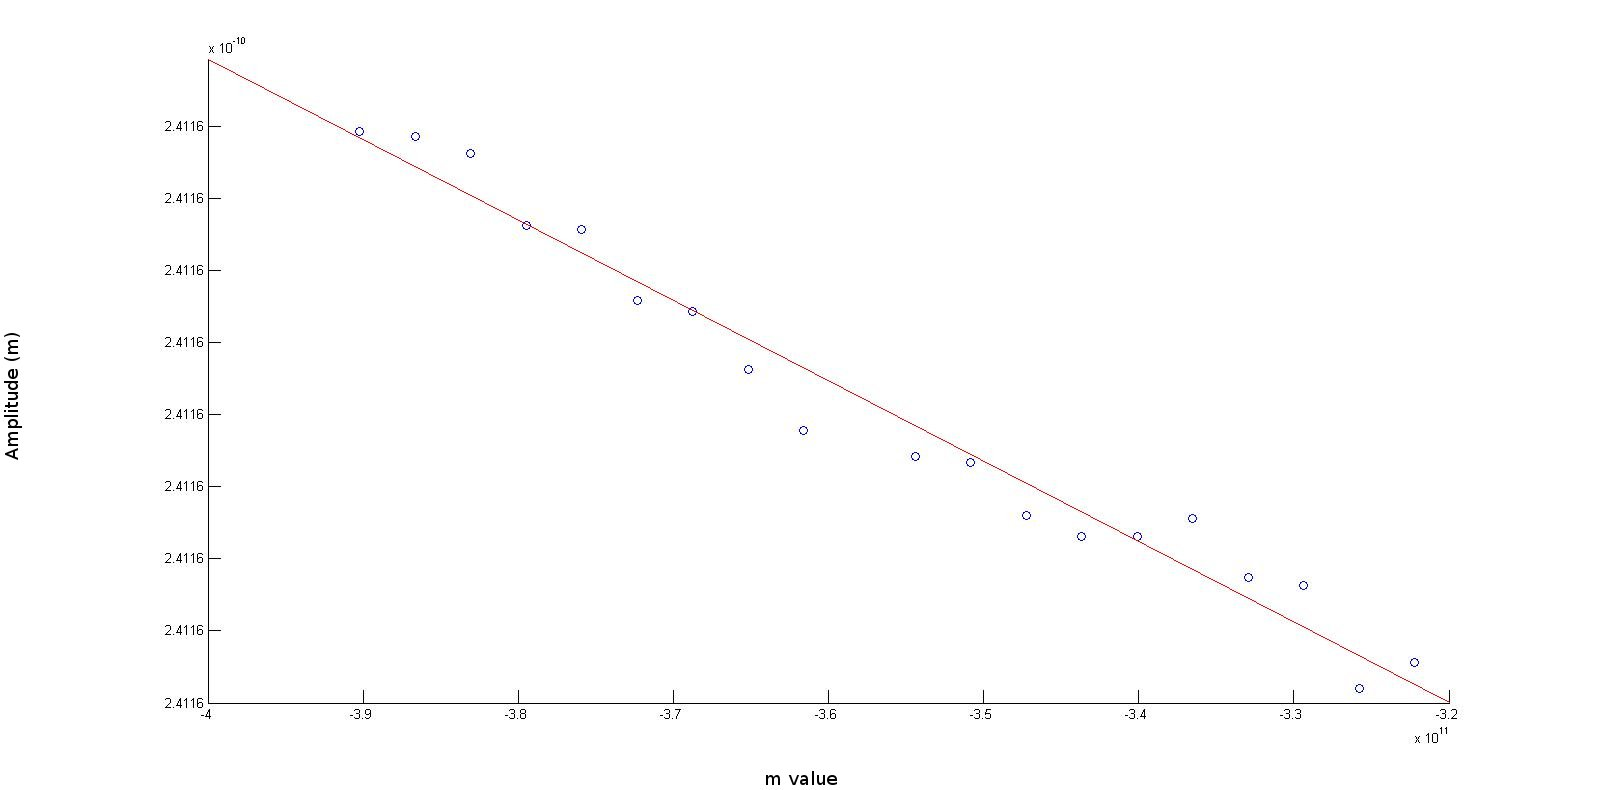
\includegraphics[scale=0.25]{images/chapter_5/forward/linear.jpg}
\caption{Linear Regression of Data with Noise}
\end{center}
\end{figure}
\begin{figure}
\begin{center}
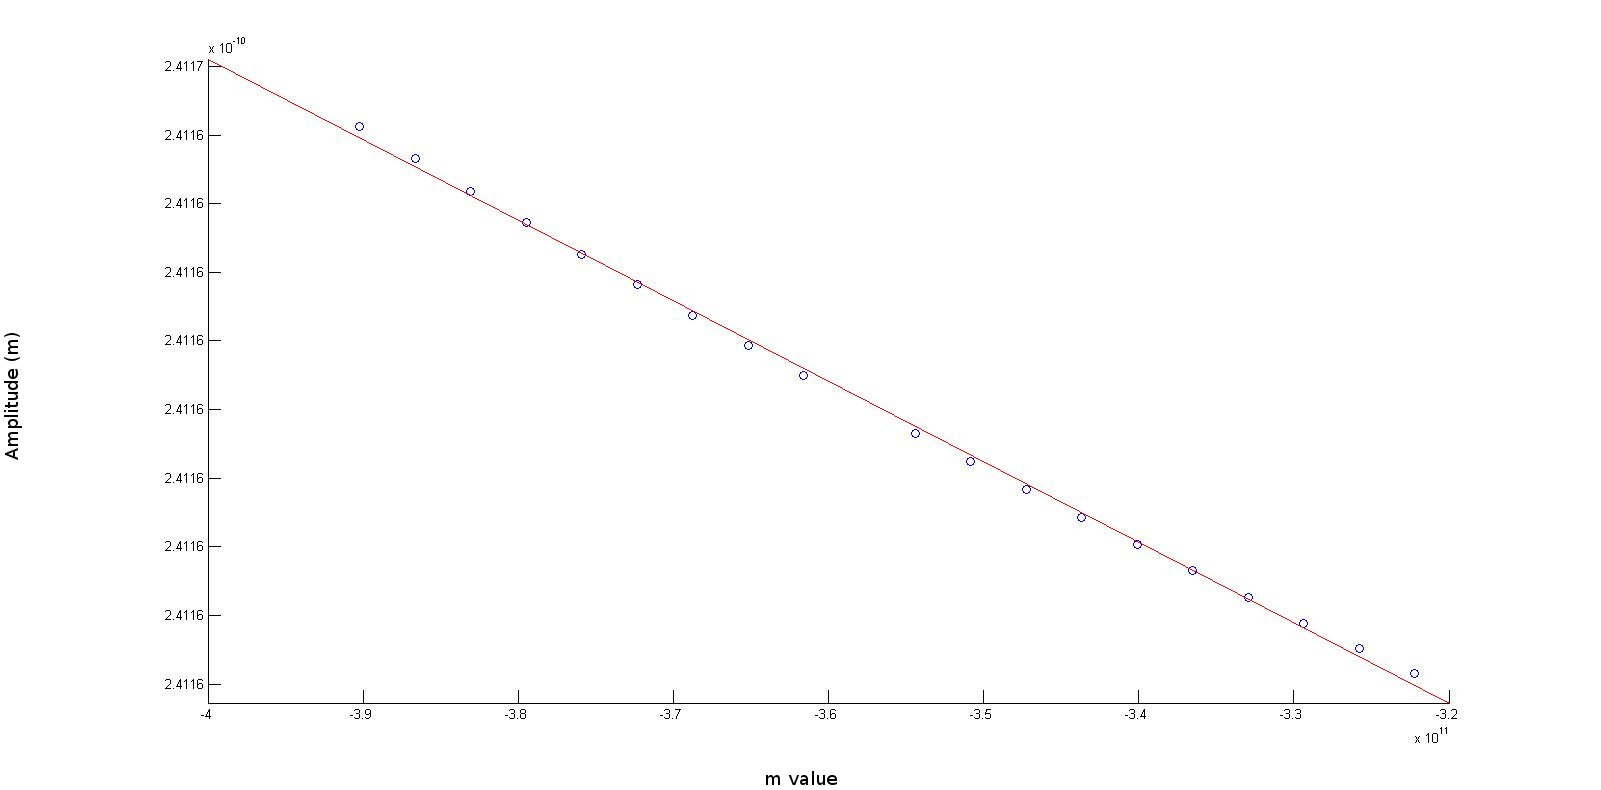
\includegraphics[scale=0.25]{images/chapter_5/forward/linear_nonoise.jpg}
\caption{Linear Regression of Data without Noise}
\end{center}
\end{figure}

\begin{figure}
\begin{center}
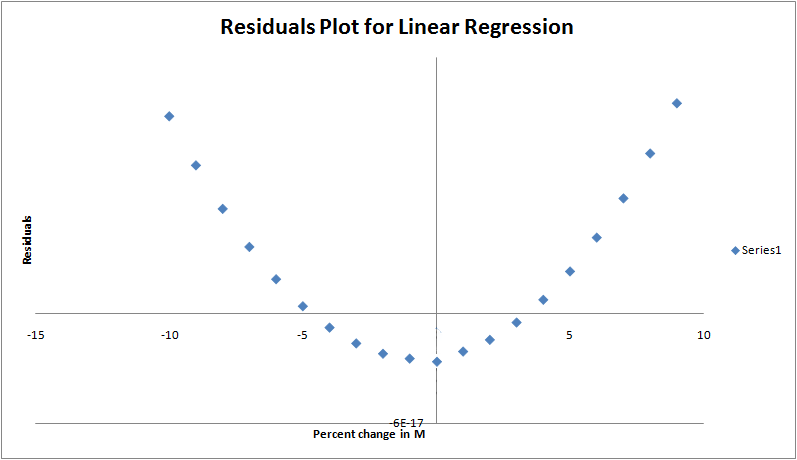
\includegraphics[scale=0.5]{images/chapter_5/forward/regression.png}
\caption{Residual Plot of Data without Noise}
\end{center}
\end{figure}

While the linear model seemed a good fit in the scenario, for a more complex case, the linear model will fail. To include the effects of the variable l, we decided to pursue a more generic approach, which is the gaussian process. This model is streamlined to negate errors as well.
\subsection{The Gaussian Process}

The gaussian process will be investigated in detail in the inversion section. A regression model using this statistical technique for the forward model proved to be quite successful and this resulted in us deciding to use the same technique for the inverse model. A support vector regression was attempted, but this method proved not be suited for this kind of a problem. Given below are the plots for the predicted values and the actual values of amplitude and normalized error.

\begin{figure}
\begin{center}
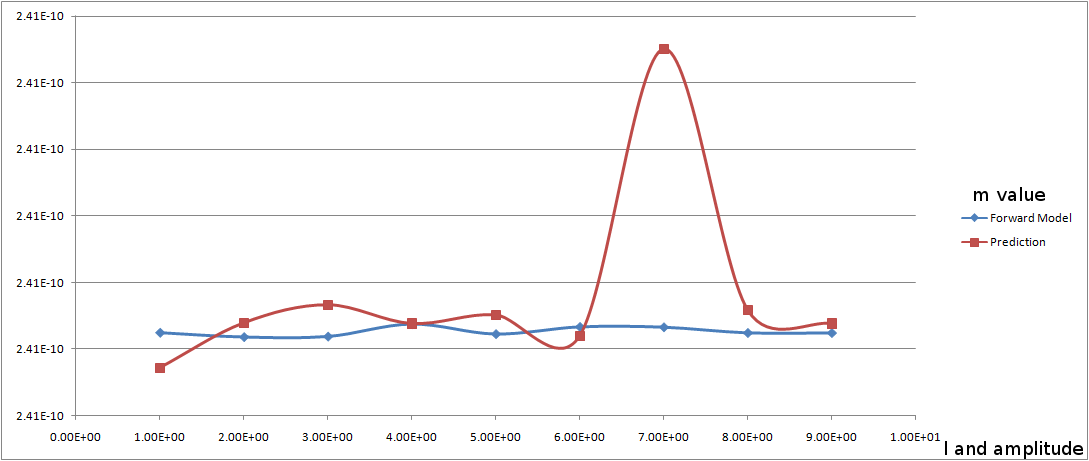
\includegraphics[scale=0.5]{images/chapter_5/forward/forward_snr_2.png}
\caption{SNR 2}
\end{center}
\end{figure}


\begin{figure}
\begin{center}
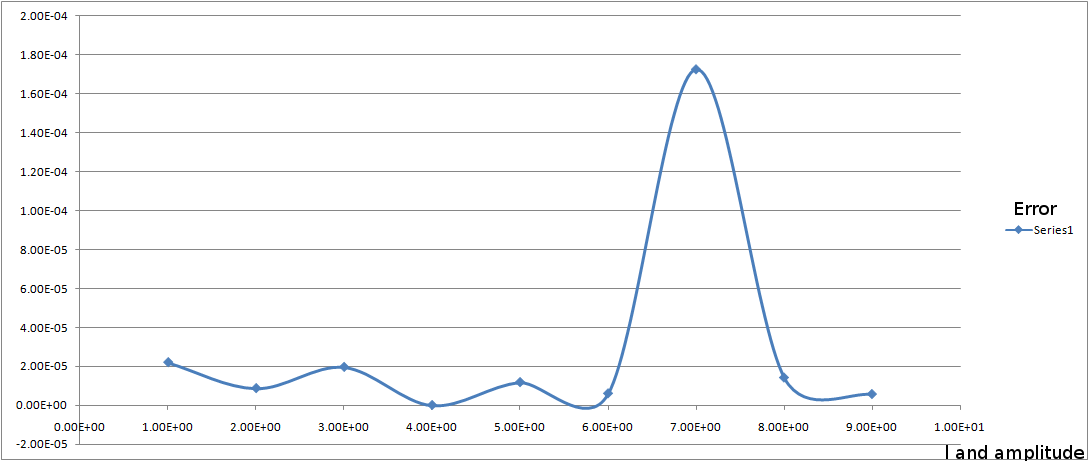
\includegraphics[scale=0.5]{images/chapter_5/forward/error_snr_2.png}
\caption{Normalized Error at SNR 2}
\end{center}
\end{figure}


\begin{figure}
\begin{center}
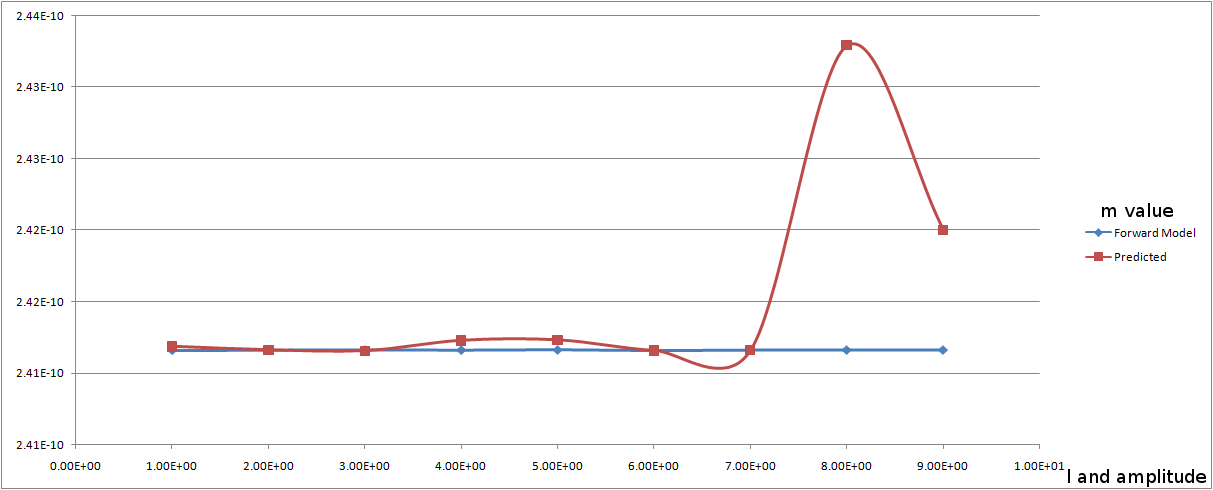
\includegraphics[scale=0.5]{images/chapter_5/forward/forward_snr_8.png}
\caption{SNR 8}
\end{center}
\end{figure}


\begin{figure}
\begin{center}
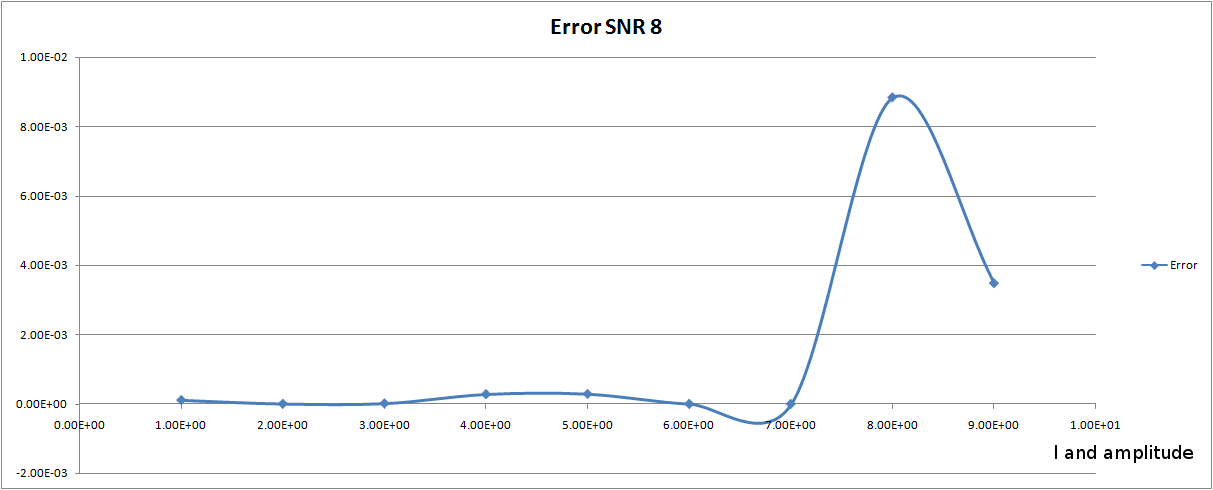
\includegraphics[scale=0.5]{images/chapter_5/forward/error_snr_8.png}
\caption{Normalized Error at SNR 8}
\end{center}
\end{figure}


\begin{figure}
\begin{center}
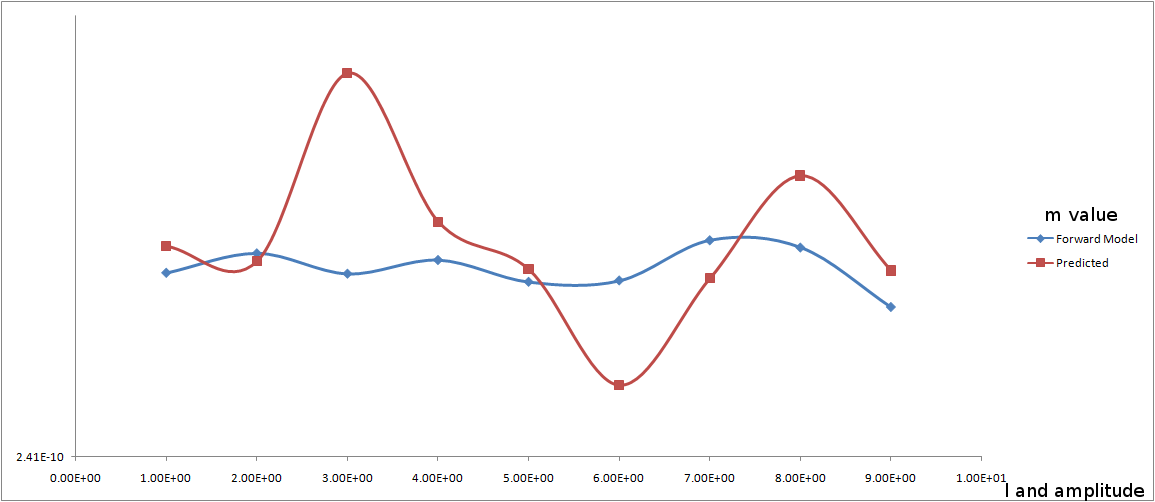
\includegraphics[scale=0.5]{images/chapter_5/forward/forward_snr_12.png}
\caption{SNR 12}
\end{center}
\end{figure}

\begin{figure}
\begin{center}
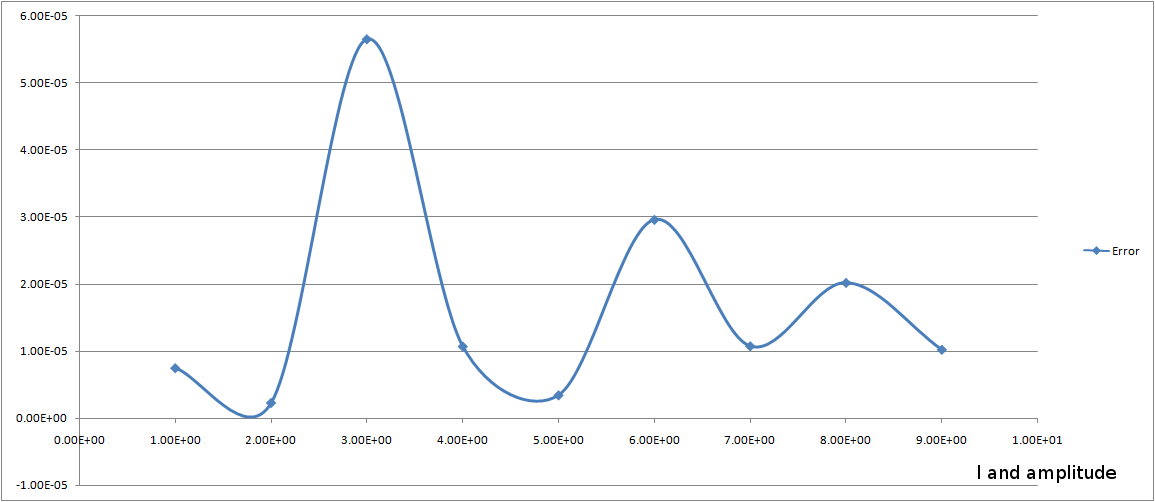
\includegraphics[scale=0.5]{images/chapter_5/forward/error_snr_12.png}
\caption{Normalized Error at SNR 12}
\end{center}
\end{figure}

\section{Statistical Techniques}
\subsection{Noisy data}
The data we have worked with till now has been data without any noise added to it. To validate the model, it is necessary to have a dataset that is contaminated with a few errors in sampling. Thus, to emulate an actual transducer's signal, we add noise to the data at Various SNRs. The results at various SNRs are compared to test the accuracy of the inverse model. Since we measure the amplitude of the resultant wave, the noise is added to the peak-to-peak amplitude value of the wave. 
\subsection{Adding Noise}
The Signal to Noise ratio for a signal can be defined as 

\begin{equation}
SNR = \frac{P_{signal}}{P_{noise}}
\end{equation}

\begin{equation}
SNR = \frac{\sigma^2_{signal}}{\sigma^2_{noise}}
\end{equation}

\begin{equation}
SNR = \frac{A^2_{signal}}{A^2_{noise}}
\end{equation}

To add noise to our amplitude signal, we calculate the power of the peak-to-peak amplitude signals, calculate the power and then add Gaussian white noise at a specific variance to match the desired Signal to Noise Ratio. In this case, we have worked with a signal to noise ratio from 2 to 20.
\subsection{The Gaussian Process}
Gaussian Processes for Machine Learning (GPML) is a generic supervised learning method primarily designed to solve regression problems.The gaussian process is a non-parametric method that works with hyperparameters. It is also a probabilistic method for regression.

The advantages of Gaussian Processes for Machine Learning are:
\begin{enumerate}
        \item The prediction interpolates the observations (at least for regular correlation models).
        \item The prediction is probabilistic (Gaussian) so that one can compute empirical confidence intervals and exceedance probabilities that might be used to refit (online fitting, adaptive fitting) the prediction in some region of interest.
        \item Versatile: different linear regression models and correlation models can be specified. Common models are provided, but it is also possible to specify custom models provided they are stationary.
\end{enumerate}
The disadvantages of Gaussian Processes for Machine Learning include:
\begin{enumerate}


        \item It is not sparse. It uses the whole samples/features information to perform the prediction.
        \item It loses efficiency in high dimensional spaces – namely when the number of features exceeds a few dozens. It might indeed give poor performance and it loses computational efficiency.
        \item Classification is only a post-processing, meaning that one first need to solve a regression problem by providing the complete scalar float precision output y of the experiment one attempt to model.

\end{enumerate}

Due to the nature of the Gaussian Process, it can be used to solve global optimization problems. From the given advantages and disadvantages of GPML, it fits perfectly for solving our inverse problem. A brief mathematical background is given for the Gaussian Process. Interested readers are requested to refer to \cite{gp} \cite{gp_tut} for a more rigorous treatment of this subject.

\subsection{Background of Gaussian Process}
The Gaussian Process instead of parametrizing the input output relationships of variables, instead assumes a prior over a distribution of functions. This helps eliminate the parametrization and associated pitfalls. Gaussian Process Treats each function as a sample from a multivariate Gaussian Distribution. Like a kernel method, it projects the finite dataset into an infinite dimensional space. To put it mathematically. Instead of parameterizing $y(\textbf{X},\textbf{w})$, we place a prior of $P(y(\textbf{x}))$. For the given data $D = {\textbf{X},\textbf{y}}$
\begin{equation}
p(\textbf{f}|\textbf{X}) = N(0,\textbf{K})
\end{equation}    
\begin{equation}
K(x,x') = E[f(x)f(x')]
\end{equation}
Now, for a GP regression, we can write $y$ as
\begin{equation}
y = f + \epsilon
\end{equation}
\begin{equation}
\epsilon = GWN(0,\sigma_e)
\end{equation}

For a test and train marginal likelihood,

\begin{equation}
p(y,y_t) = N(0, K_{N+T}) + \sigma^2_e \textbf{I}
\end{equation}

\begin{equation}
p(y_T | y) = N(\mu_T, \Sigma_T)
\end{equation}

The solutions to this formulation are beyond the scope of this dissertation and the reader is requested to consult the references mentioned above. This problem now becomes an optimization problem to minimize log likelihood. This gives us our solution.
\section{Discussion and Results}

From the results and the limited plots shown in the figures below, it is evident that the Gaussian Process acts as a very good statistical estimator for this case. The inversion of model parameters is quite successful and thus even for complex use cases will do a good job. Due to the nature of the techniques employed, the solutions obtained are close to the global optima, and thus quite accurate.

\begin{figure}
\begin{center}
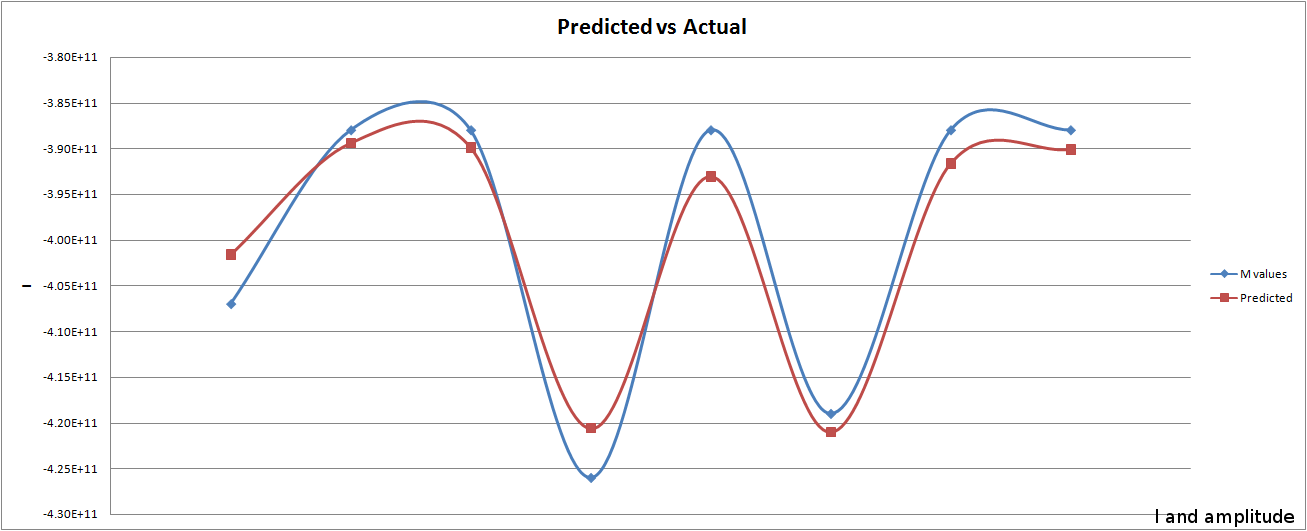
\includegraphics[scale=0.5]{images/chapter_5/inverse/pred_snr_2.png}
\caption{Prediction of Value of M at SNR 2}
\end{center}
\end{figure}


\begin{figure}
\begin{center}
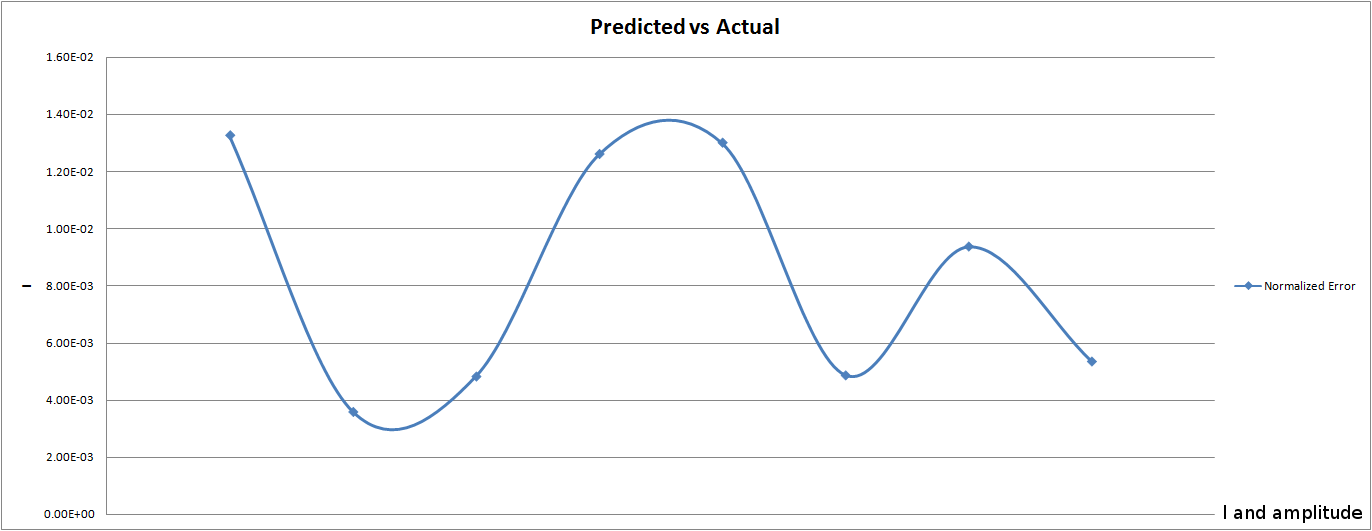
\includegraphics[scale=0.5]{images/chapter_5/inverse/error_snr_2.png}
\caption{normalized Error of M at SNR 12}
\end{center}
\end{figure}


\begin{figure}
\begin{center}
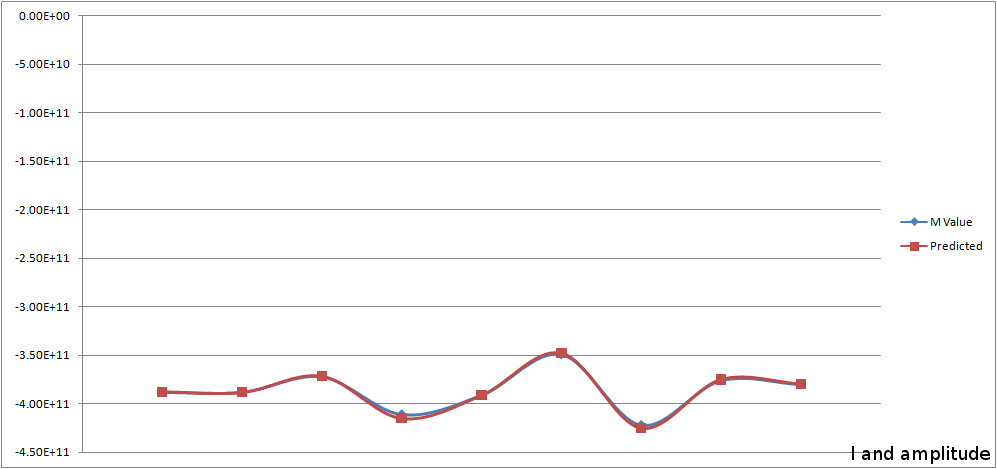
\includegraphics[scale=0.5]{images/chapter_5/inverse/pred_snr_8.png}
\caption{Prediction of Value of M at SNR 8}
\end{center}
\end{figure}


\begin{figure}
\begin{center}
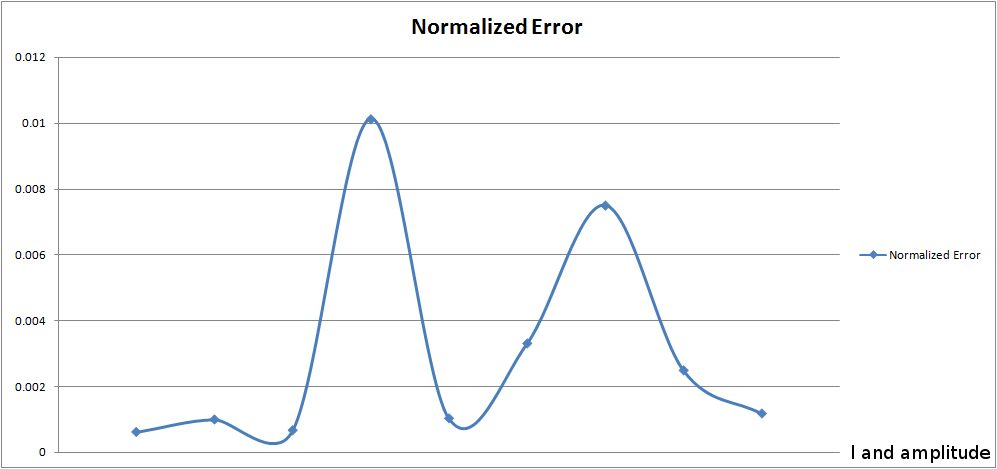
\includegraphics[scale=0.5]{images/chapter_5/inverse/error_snr_8.png}
\caption{normalized Error of M at SNR 8}
\end{center}
\end{figure}


\begin{figure}
\begin{center}
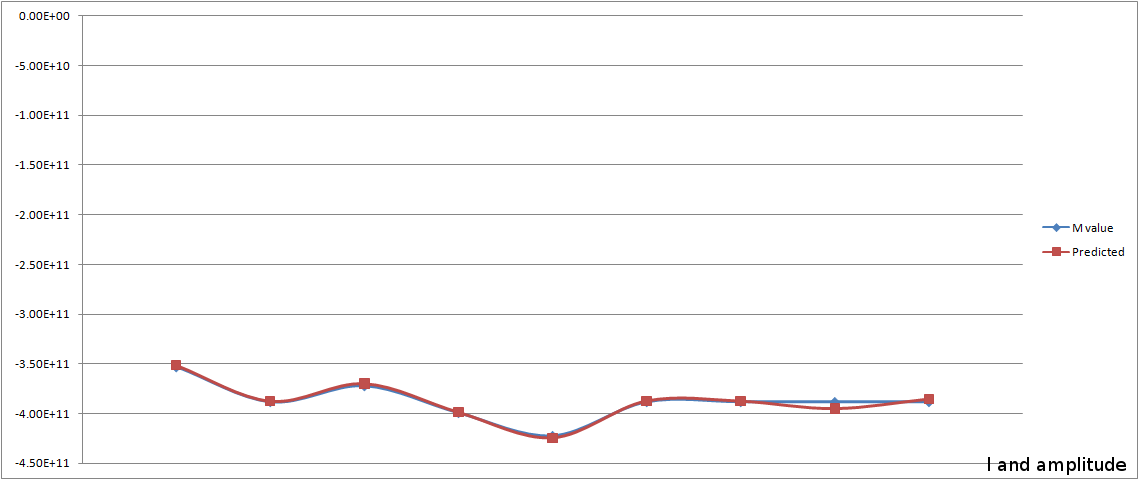
\includegraphics[scale=0.5]{images/chapter_5/inverse/pred_snr_12.png}
\caption{Prediction of Value of M at SNR 2}
\end{center}
\end{figure}


\begin{figure}
\begin{center}
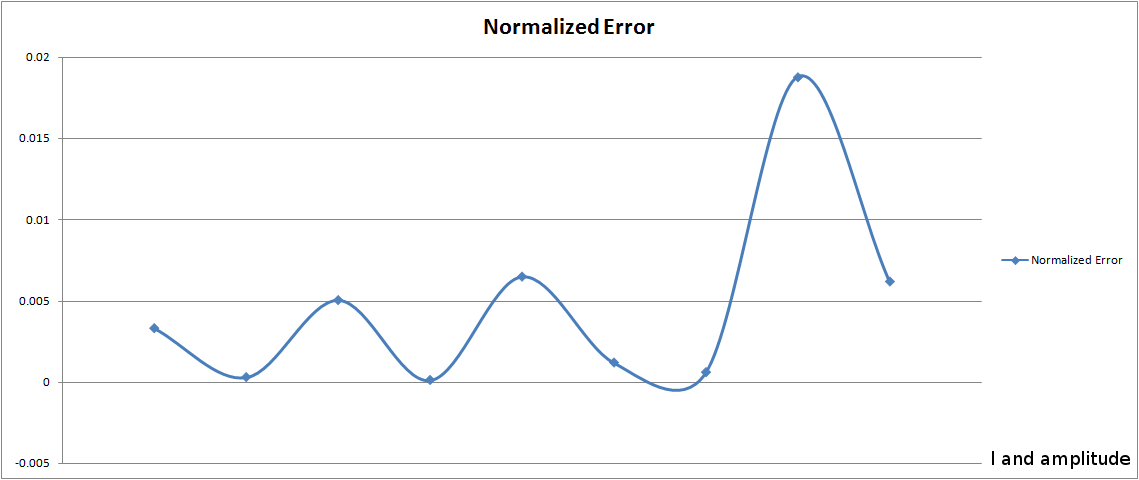
\includegraphics[scale=0.5]{images/chapter_5/inverse/error_snr_12.png}
\caption{normalized Error of M at SNR 12}
\end{center}
\end{figure}

\subsection{Caveats}
There are quite a few caveats to the inversion model produced here. Firstly, the case we have chosen to model happens to be a very specific case of a very difficult to solve generic problem. In this case, the model parameters luckily end up being independent of each other, which makes our task much easier. For a more complicated use case, the model parameters might be correlated which will result in difficulties. The inversion technique we have used has proven to be quite efficient.
